% !TEX root = ../thesis.tex

In this chapter, we focus on the problem of approximating the smoothing distributions for a Hidden Markov Model (HMM) with continuous state-space.
We assume that a sequence of empirical densities approximating the filtering distributions has already been obtained through a particle filtering step.
We had seen at point \ref{bg:particle-smoothing} that the \emph{forward filtering backward smoothing} (FFBS) algorithm can produce an approximation to the smoothing distributions by recycling a particle filter and updating its weights.  As shown in point \ref{bg:particle-smoothing}, the FFBS algorithm has quadratic complexity and may suffer from the lack of resampling step if the smoothing distribution and the filtering distribution have significantly different support. 

In this chapter, we introduce a class of algorithms that can be obtained from another factorisation of the smoothing distributions than that used to obtain the FFBS. We also introduce algorithms with a computational complexity that is sub-quadratic in $N$ and compare these algorithms in numerical experiments.

%%%%%%%%%%%%%%%%%%%%%%%%%%%%
\section{Two Filter Smoothing}


\subsection{\label{point:TFS}Two filter formula}
An alternative to the FFBS approach is to exploit the \emph{two filter formula}. 
To derive it, note that the smoothing distribution can be written in the following way using Bayes' formula:
%
\eqa{
	p(x_t\st y_{1:T})&=& {p(x_t,y_{1:t-1},y_{t:T})\over p(y_{1:T})}.\nn
	}
% 
Then, exploiting the conditional dependences of the HMM, we get
%
\eqa{
	p(x_t\st y_{1:T}) 	
		&\propto& p(y_{t+1:T}\st x_t,x_{t+1},y_t)p(y_t\st x_t,x_{t+1})
\nn\\
		&\propto& p(x_t\st y_{1:t-1})p(y_{t:T}\st x_t).	\label{eq:TFS}
}
%
This last factorised form is the two filter formula which leads to the \emph{two filter smoothing} (TFS) algorithm \citep{bresler86, kitagawa96}. 
The first term in \eqref{eq:TFS} is the prediction density (PD), 
the second term $p(y_{t:T}\st x_{t})$ is called the \emph{backward information filter} (BIF). To simplify developments we introduce the following non-standard notations for the predictive density and the backward information filter:\check{jul16}
%
\eqa{
	\pd_{t}(x_{t}) \esp:=\esp p(x_{t}\st y_{1:t-1}), \quad\text{and}  \quad \bif_{t}(x_{t}) \esp:=\esp p(y_{t:T}\st x_{t}).
}
%
The prediction density is obtained by integrating the filtering density multiplied by the transition density:
%
\eqa{
	\pd_{t}(x_{t}) &=& \int p(x_{t}\st x_{t-1})p(x_{t-1}\st y_{1:t-1})\dx_{t-1}.\label{eq:pred-dens}
}
%
an approximation to the prediction density can therefore easily be obtained by plugging a particle representation of the filtering density in \eqref{eq:pred-dens}. \check{jul16, july5}
%%%%%%%%%%%%%%%%%%%%%%%%%%
\subsection{Targeting the backward information filter}
The backward information filter cannot be directly targeted in a SMC framework in general as it may not be proportional to a distribution in $x_{t}$. 
In \citet{briers10}, the authors therefore suggest to introduce a sequence of artificial \emph{normalisation densities} $\{\gamma_{t}\}_{t=1}^{T}\in\mathcal P(\mathcal X)$ such that, for each step $t$, the product of $\gamma_{t}$ and $\bif_{t}$ is normalisable. 
In other words, the normalising distribution $\gamma_{t}$ allows to define a \emph{normalised backward information filter} in $\mathcal P(\mathcal X)$ with
%
\eqa{
	\tbif_{t}(x_{t}) &:=& Z\inv_{t}\gamma_{t}(x_{t})\bif_{t}(x_{t})
}
%
for some normalising constant $Z\inv_{t}$.\check{july5}
Any $\gamma_{t}\in\mathcal P(\mathcal X)$ can be chosen as long as it verifies the \emph{support condition} i.e.: as long as its support covers that of the backward information filter:
%
\eqa{	
	\bif_t(x_t) &>&0 \quad\Longrightarrow\quad \gamma_{t}(x_{t})\esp>\esp 0. \label{eq: tech condition normalisation density}	
}
%
In order to target the sequence of normalised BIF in a SMC framework, it is useful to show that it verifies a factorisation structure similar to that of the filtering distribution. For this, we start by noting that
%
\eqa{		
	p(y_{t:T}\st x_{t},x_{t+1}) 
		&=& p(y_{t+1:T}\st x_{t},x_{t+1},y_{t})p(y_{t}\st x_{t},x_{t+1})\nn\\
		&=& p(y_{t}\st x_{t}) \bif_{t+1}(x_{t+1}). \label{back rec 1}	
}
%
On the other hand, we also have that
%
\eqa{		
	p(y_{t:T}\st x_{t},x_{t+1}) 	
		&=& {p(y_{t:T},x_{t},x_{t+1})\over p(x_{t+1}\st x_{t})p(x_{t})}\nn\\
		&=&{p(x_{t+1}\st x_{t},y_{t+1:T})\text{BIF}_{t}(x_{t})\over p(x_{t+1}\st x_{t})},	\label{back rec 2}
}
%
where we have used the conditional independence structure of the HMM. 
Combining \eqref{back rec 1} and \eqref{back rec 2} then leads to\check{july5}
%
\eqa{	
	\bif_{t}(x_{t}) p(x_{t+1}\st x_{t},y_{t+1:T}) &=& p(y_{t}\st x_{t})p(x_{t+1}\st x_{t})\bif_{t+1}(x_{t+1}). 	\label{eq:tfs-bif2}
}
%
If we now introduce the normalisation densities $\gamma_{t}$ and $\gamma_{t+1}$ and the corresponding normalisation constants $Z_{t}$ and $Z_{t+1}$ in \eqref{eq:tfs-bif2} we get\check{july5}
%
\eqa{	 
	\tbif_{t}(x_{t})p(x_{t+1}\st x_{t},y_{t+1:T}) &=& 
		{Z_{t+1}\gamma_{t}(x_{t})\over Z_{t}\gamma_{t+1}(x_{t+1})}p(y_{t}\st x_{t})p(x_{t+1}\st x_{t})\tbif_{t+1}(x_{t+1}).		\nn
}
%
By construction of the normalisation densities, we can integrate the previous expression over $x_{t+1}$ to obtain
%
\eqa{		
	\tbif_{t}(x_{t}) &\propto& {\gamma_{t}(x_{t})}p(y_{t}\st x_{t})\int p(x_{t+1}\st x_{t}){\tbif_{t+1}(x_{t+1})\over \gamma_{t+1}(x_{t+1})}\dx_{t+1}.	\nn
}
%
Noting that $\bif_{T}(x_{T})=p(y_{T}\st x_{T})$ and iterating brings
%
\eqa{		
	\tbif_{t}(x_{t}) &=& \int {\gamma_{t}(x_{t})}\prod_{\ell=t}^{T-1}p(x_{\ell+1}\st x_{\ell})\prod_{k=t}^{T}p(y_{k}\st x_{k})\dx_{t+1:T}.	\nn
}
%
We can thus define a joint distribution $\tbif_{t}(x_{t:T})$ as the integrand of the above expression with the following sequential structure:
\eqa{		\tbif_{t}(x_{t:T}) &\propto& {\gamma_{t}(x_{t})p(x_{t+1}\st x_{t})p(y_{t}\st x_{t})\over \gamma_{t+1}(x_{t+1})}\tbif_{t+1}(x_{t+1:T}),	\label{recursion joint BIF}}
which lends itself well to the SMC framework with the optimal proposal:\check{jul16,july5}
%
\eqa{
	q^{\text{opt}}_{t}(x_{t}\st x_{t+1}) &\propto& {\gamma_{t}(x_{t})p(x_{t+1}\st x_{t})p(y_{t}\st x_{t})\over \gamma_{t+1}(x_{t+1})}.
}
%
%%%%%%%%%%%%%%%%%%%%%%%%%%%%%
\subsection{\label{introTFS}Two filter smoothing algorithm}
Plugging a particle representation of the filtering distribution in \eqref{eq:pred-dens}, the prediction density can be approximated by
%
\eqa{
	\widehat\pd_t(x_t)  &=& \sum_{i=1}^{N} w^{(i)}_{t-1}p(x_{t}\st X^{(i)}_{t-1}).	
\label{eq PDhat}	
}
%
Correspondingly, we can consider a particle representation of the normalised BIF obtained by following a backward particle filter with $M$ particles on \eqref{recursion joint BIF}. 
%The non-standard notation $\pd_{t}$ as well as the notations introduced below for the backward information filter will make the discussion of the TFS algorithm simpler and less cluttered. The backward information filter $\bif_t(x_t):=p(y_{t:T}\st x_{t})$ is not necessarily proportional to a distribution in $x_{t}$ and can thus not be directly targeted in a SMC context. However, one can define an auxiliary quantity by pre-multiplying the backward information filter by an artificial \emph{normalisation density} $\gamma_{t}(x_{t})$ such that the product
%%
%\eqa{		
%	\tbif_t(x_t) &:=& Z_{t}\inv{\gamma_{t}(x_{t}) p(y_{t:T}\st x_t)},		\label{def normalised BIF}
%}
%%
%is a distribution in $x_{t}$ (with $Z_{t}$ a normalisation constant) and can thus be targeted in the SMC framework \citep{briers10}.\check{jun24} 
%We will refer to these densities as \emph{normalisation densities}. The $\tbif_{t}$ are distributions and can be targeted in a SMC framework. 
Let us denote these by $\widehat\tbif_{t}$ with weights $\tilde w_{t+1}^{(j)}$ and particles $\tilde X^{(j)}_{t+1}$, i.e.:
%
\eqa{		
	\widehat\tbif_t(x_t) &=& \sum_{j=1}^{M} \tilde w^{(j)}_{t+1} \delta_{\tilde X^{(j)}_{t+1}}(x_{t}).
	} 
%
By dividing these by the corresponding normalisation density $\gamma_{t}$, we can obtain approximations to the original BIF:
%
\eqa{		
	\widehat\bif_t(x_t) &=& { \widehat\tbif_t(x_t)/  \gamma_{t}(x_{t})}.	\nn
}
%
Combining both the estimators of the prediction density and the backward information filter at step $t$, we can obtain a particle representation of the smoothing distribution with\check{jul5}
%
\eqa{		
	\hat{p}(x_{t}\st y_{1:T}) &=& \zeta_{t}\inv\widehat\pd_t(x_t)\widehat\bif_t(x_t)	, \label{first smoothing estimator}	
	}
%
where $\zeta_{t}$ is a normalisation constant.
That is a mixture of $NM$ terms and a further step may be desirable to reduce the number of components in the resulting representation of the smoothing distribution.
In particular, if we take $M=N$, at each step we have to consider a mixture with a quadratic number of terms in $N$ and this, independently of the choice of normalising densities meaning that the algorithm has inherently a quadratic complexity. We consider this choice in what follows.\check{jul16,jul5}
%Note that since both the predictive density and the normalised BIF have been approximated using $N$ particles, the above estimator is a mixture of $N^{2}$ components and a further resampling step can be applied to reduce it to a mixture of only $N$ components. %\add{This is what Fearnhead does}

%Another comment that we can make at this point is that the form of the estimator in \eqref{first smoothing estimator} suggests taking as normalisation densities the estimator of the prediction densities. \\

%We will show explicitly how to implement the two filter smoothing algorithm with a near-ideal normalisation density in \hyperref[sec:TFS]{section \ref*{sec:TFS}}. 


%\todofr{
%\begin{itemize}
%	\item Add here the algorithm
%	\item add short discussion (complexity, choice of normalisation)
%\end{itemize}
%}


%%%%%%%%%%%%%%%%%%%%%
\section{Backward Information Smoothing}
In this section, we explore the choice of normalisation densities and suggest using an approximation to the predictive density. It came to our knowledge that this choice had in fact also been studied independently and earlier than this work by \citet{taghavi12}. 
We show how the complexity of the resulting algorithm is quadratic in the number of particles. 
We also discuss two modified versions with sub-quadratic complexity. 
The first one, inspired by \citet{fearnhead10} and also discussed by \citet{taghavi12}, has linear complexity but the resulting estimators are not consistent. 
The second one, inspired by our paper \citep{lienart15}, has complexity $\mathcal O(NM)$ where $M$ is sub-linear in $N$ and leads to consistent estimators. \check{jul16}

%%%%%%%%%%%%%%%%%%%%%%%
\subsection{Choice of normalisation densities}
The choice of normalisation densities in the TFS algorithm is, in theory, only constrained by the support condition \eqref{eq: tech condition normalisation density}. However, the quality of the corresponding estimators for a finite sample size depends significantly on it. 
Combining \eqref{eq:TFS} and \eqref{recursion joint BIF}, we get
%
\eqa{
	p(x_{t}\st y_{t:T}) &\propto& {\pd_{t}(x_{t})\over \gamma_{t}(x_{t})} \int \tbif_{t}(x_{t:T}) \dx_{t+1:T}\nn
}
%
so that we can write
%
\eqa{		
	p(x_{t:T}\st y_{1:T}) &\propto& {\pd_{t}(x_{t})\tbif_{t}(x_{t:T})\over \gamma_{t}(x_{t})}	\label{normalised BIF and partial joint}.
}
%
This expression suggests picking $\gamma_{1}$ to be the prior distribution on the first state $\pi_{0}(x_{1})$ since that leads directly to 
%
\eqa{		
	p(x_{1:T}\st y_{1:T}) &=& \tbif_{1}(x_{1:T}).	\label{full joint and first bif}
	}
%
The last two equations \eqref{normalised BIF and partial joint} and \eqref{full joint and first bif} are crucial for the rest of the analysis. The first one suggests that if we pick $\gamma_{t}$ to be close to the predictive density then, then each term $\tbif_{t}(x_{t:T})$ forms an estimator for the partial joint smoothing densities $p(x_{t:T}\st y_{1:T})$; the second one indicates that upon selecting $\gamma_{1}$ to be the prior for the initial state, we end up targeting exactly the joint distribution of interest, no matter which admissible sequence $\{\gamma_{t}\}_{t=2}^{T}$ we picked earlier. \check{jul16}

This suggests to build a good estimator of the prediction density, based partly or entirely on a particle estimator of the filtering density; use it as normalisation density and target the corresponding normalised BIF recursively. 
We explored this idea and showed that it significantly outperforms the default choice used in \citep{briers10, fearnhead10} where the authors suggest also taking $\gamma_{1}$ as the prior $\pi_{0}$ and the subsequent $\gamma_{t}$ by propagating this through the dynamic of the HMM i.e.:
%
\eqa{
	\gamma_{t}(x_{t}) &=& \int p(x_{t}\st x_{t-1})\gamma_{t-1}(x_{t-1}) \mathrm dx_{t-1}\label{eq:choice-norma-bad}
}
%
Note that this choice also suffers from a tractability issue in a system with dynamic that is more complex than the linear and Gaussian one considered in \citep{fearnhead10} where, in any case, the optimal Kalman smoother should be preferred. We show in the appendix (point \ref{app:normalising-density-fearnhead-lg}) how this normalising density can be obtained in the case of a simple linear Gaussian dynamic.\check{jul16}

Upon selecting $\gamma_{t}$ to be the approximation of the predictive density \eqref{eq PDhat} based entirely on a a particle estimator of the filtering density, we get what Taghavi calls the \emph{backward informations smoothing} (BIS) algorithm \citet{taghavi12}. This choice verifies the support condition \eqref{eq: tech condition normalisation density} provided the support  of $p(x\st z)$ covers the support of the BIF. Typically, the support of $p(x\st z)$ is the whole space $\mathcal X$ which guarantees this.

The optimal importance function for targeting the corresponding normalised BIF is obtained by considering \eqref{recursion joint BIF} with this specific choice of normalising density:\check{jul16, jul2}
\eqa{		\tilde q^{\text{opt}}_{t}(x_{t}\st \tilde X^{(j)}_{t+1}) &\propto & {\hpd_{t}(x_{t})\over \hpd_{t+1}(\tilde X^{(j)}_{t+1})} p(\tilde X^{(j)}_{t+1}\st x_{t})p(y_{t}\st x_{t}),\label{eq:opt-prop-bif}}
where the $\{\tilde X_{t+1}^{(j)}\}_{j=1}^{N}$ are the particles from the previous smoothing step. These steps are illustrated in algorithm \ref{alg:bisquad}.\check{jul5}

%
\begin{algorithm}[!h]\small
	\caption{\label{alg:bisquad}\dblue{\emph{\small Backward information smoother with quadratic complexity}}}
	\begin{algorithmic}[1]
		\State run a PF targeting $\{p(x_{t}\st y_{1:t})\}_{t=1}^{T}$ with $N$ particles $\{X^{(i)}_{t}, w^{(i)}_{t}\}_{t,i=1}^{T,N}$
		\For{$t=T-1:2$}
			\State sample $\tilde X^{(j)}_{t}\simiid \tilde q_{t}(\cdot\st \tilde X^{(j)}_{t+1})$ with $\tilde q_{t}\approx \tilde q_{t}^{\text{opt}}$ for $j=1,\dots,N$
			\State update and normalise the weights $\tilde w^{(j)}_{t}\propto \tilde\alpha^{(j)}_{t}\tilde w^{(j)}_{t+1}$
		\EndFor
		\State same operations for $t=1$ but with $\tilde q^{\text{opt},i,j}_{1} \propto \pi_{0}(x_{1})p(\tilde X^{(j)}_{2}\st x_{1})p(y_{1}\st x_{1})/\hpd_{2}(\tilde X^{(j)}_{2})$\\

		\Return weighted set of particles $\{\tilde X^{(j)}_{1:T}, \tilde w^{(j)}_{1:T}\}$
	\end{algorithmic}
\end{algorithm}
%

At each step $t$ and for each particle $j$, the algorithm \ref{alg:bisquad} ideally requires sampling a particle from $\hpd_{t}(x_{t})p(\tilde X^{(j)}_{t+1}\st x_{t})p(y_{t}\st x_{t})$ which is a mixture of $N$ terms. Additionally, computing the updating factors for the weights requires computing a sum of $N$ terms $\hpd_{t+1}(\tilde X_{t+1}^{(j)})$. Provided we use $N$ particles to target the BIF, the complexity of the BIS algorithm is therefore inherently quadratic in the number of particles. This is the same computational complexity as that of the FFBS algorithm.\check{jul16, jul5}

As it is not trivial in general to sample from $p(\tilde X^{(j)}_{t+1}\st x_{t})p(y_{t}\st x_{t})$, let alone when it is combined with $\hpd_{t}(x_{t})$, a possibility akin to the bootstrap proposal for the particle filter is to simply sample from $\hpd_{t}(x_{t})$. The disadvantage is that this choice doesn't take into account all the information available (contained in $\tilde X^{(j)}_{t}$ and $y_{t}$). Assuming we can sample easily from the transition distribution, sampling from $\hpd_{t}$ can be done easily in two steps: first sample an index $i^{\star}\sim \mathcal M(w^{(1)}_{t-1}, \dots, w^{(N)}_{t-1})$ where $\mathcal M$ denotes a multinomial distribution and then sample from the corresponding term $p(x_{t}\st X^{(i^{\star})}_{t-1})$. The update factor is then given by
%
\eqa{
	\tilde\alpha^{(j)}_{t} &=& { p(\tilde X^{(j)}_{t+1} \st \tilde X^{(j)}_{t})p(y_{t}\st \tilde X^{(j)}_{t}) \over \hpd_{t+1}(\tilde X^{(j)}_{t+1})},
}
%
which has linear complexity in the number of particles for each $j$ so that, as expected, the \emph{bootstrap backward information smoother} also has quadratic complexity.\check{jul16}

%%%%%%%%%%%%%%%%%%%%%%%%
\subsection{BIS with linear complexity}
%
We have shown that the BIF algorithm is inherently quadratic in the number of particles given the form of the optimal proposal \eqref{eq:opt-prop-bif}. A statistically equivalent way of writing the optimal sampling step is to suggest sampling $N$ particles from a mixture of $N^{2}$ terms: 
%
\eqa{
	\tilde X^{(j)}_{t} &\simiid & \tilde q^{\text{mix}}_{t} \esp\propto\esp \sum_{i,j=1}^{N} {w^{(i)}_{t-1} \tilde w^{(j)}_{t+1} \over s^{(j)}_{t+1}} p(x_{t}\st X^{(i)}_{t-1})p(y_{t}\st x_{t})p(\tilde X^{(j)}_{t+1}\st x_{t}),
} 
where $s^{(j)}_{t+1}=\sum_{k=1}^{n}w^{(k)}_{t}p(\tilde X^{(j)}_{t+1}\st X^{(k)}_{t})$. Since this is equivalent to sampling from the optimal proposal, no reweighing step is needed, provided we can sample exactly from the mixture.\check{jul16, jul6}
 
Sampling from such a mixture can be done in two steps: first, sample a pair of labels $(i^{\star},j^{\star})$ from a multinomial distributions with $N^{2}$ weights $\beta^{(i,j)}_{t}$ corresponding to the weight of the component $(i,j)$ relative to the whole mixture $q_{t}^{\text{mix}}$; second, sample from the component $(i^{\star},j^{\star})$. 
Of course this does not simplify the problem: we still have to sample $N$ pairs of indices from a multinomial with $N^{2}$ pair which is still quadratic in $N$ and, additionally, computing the mixture component weights $\beta^{(i,j)}_{t}$ is intractable in general. \check{jul16,jul10}

An approximation suggested first by \citet{briers05} in the wider context of sampling from products of mixtures and exploited by \citet{fearnhead10, taghavi12} in the context of the TFS algorithm is to approximate $i$ and $j$ independently by representing $\beta^{(i,j)}_{t}\approx \beta^{(i)}_{t}\beta^{(j)}_{t}$. The simplest form for this approximation, is to use $\beta^{(i)}_{t} = w^{(i)}_{t-1}$ and $\beta^{(j)}_{t}=\tilde w^{(j)}_{t+1}$. 

Since sampling from a given component $p(x_{t}\st X^{(i^{\star})}_{t-1})p(y_{t}\st x_{t})p(\tilde X^{(j^{\star})}_{t+1}\st x_{t})$ may still be intractable, we can resort to importance sampling for that term as well and compute the corresponding importance weight $\tilde w_{t}^{(j)}$ as a result.
With this approach, sampling the indices is now an operation with linear computational complexity in the number of particles and the resulting algorithm consequently also enjoys linear complexity. 
The steps are illustrated in algorithm \ref{alg:bis-linear}. \check{jul16}
%
\begin{algorithm}[!h]\small
	\caption{\label{alg:bis-linear}\dblue{\emph{\small BIS with linear complexity}}}
	\begin{algorithmic}[1]
		\State run a particle filter targeting $\{p(x_{t}\st y_{1:t})\}_{t=1}^{T}$ with $N$ particles $\{X^{(i)}_{t}, w^{(i)}_{t}\}_{t,i=1}^{T,N}$
		\State set $\{\tilde X^{(j)}_{T},\tilde w^{(j)}_{T}\}_{j=1}^{N}\leftarrow \{X^{(i)}_{T},w^{(i)}_{T}\}_{i=1}^{N}$
		\For{$t=T-1:2$}
			\State sample $N$ pairs of indices with $i^{\star}_{1:N} \simiid \mathcal M(\beta^{(i)}_{t})$ and $j^{\star}_{1:N}\simiid \mathcal M(\beta^{(j)}_{t})$
			\For{$k=1:N$}
				\State sample $\tilde X^{(k)}_{t}\sim \tilde  q_{t} \approx \tilde q_{t}^{\text{opt}, i^{\star}_{k}, j^{\star}_{k}}(x_{t}) \propto p(x_{t}\st X^{(i^{\star}_{k})}_{t-1})p(\tilde X^{(j^{\star}_{k})}_{t+1}\st x_{t})p(y_{t}\st x_{t})$
	    			\State compute the unnormalised weights $\tilde w^{(k)}_{t} \propto \tilde q^{\text{opt}, i^{\star}_{k},j^{\star}_{k}}_{t}(\tilde X^{(k)}_{t})/\tilde q_{t}(\tilde X^{(k)}_{t})$
			\EndFor
			\State normalise the weights (and resample if necessary)
		\EndFor
	\State same operations for $t=1$ but with $\tilde q^{\text{opt},i,j}_{1} \propto \pi_{0}(x_{1})p(\tilde X^{(j)}_{2}\st x_{1})p(y_{1}\st x_{1})$\\
	\Return weighted set of particles $\{\tilde X^{(j)}_{1:T}, \tilde w^{(j)}_{1:T}\}_{j=1}^{N}$
	\end{algorithmic}
\end{algorithm}

Note that, in algorithm \ref{alg:bis-linear}, a resampling step can also be introduced if the ESS drops below a fixed admissible threshold as with the particle filtering algorithm. 
Note also that the approximation inspired by \citet{briers05} used in this algorithm is what leads to an algorithm with linear complexity but also results in estimators that do not enjoy the consistency property of standard importance sampling estimators.\check{jul13}

%%%%%%%%%%%%%%%%%%%%%%%%%%%%%
\subsection{Consistent BIS with sub-quadratic complexity}
%
We discussed earlier the bootstrap BIS with quadratic complexity where one samples from the approximation to the predictive density $\hpd_{t}$.
This can in fact be simplified by compressing the representation of the particle filter from $N$ particles to $M$ particles by resampling. Taking $M$ to be sub-linear in $N$ (e.g.: $M=\mathcal O(\log N)$), the overall algorithm is $\mathcal O(TMN)$ and sub-quadratic in $N$.

%
\begin{algorithm}[!h]\small
	\caption{\label{alg:bis-sublin}\dblue{\emph{\small Bootstrap BIS with sub-quadratic complexity}}}
	\begin{algorithmic}[1]
		\State run a PF targeting $\{p(x_{t}\st y_{1:t})\}_{t=1}^{T}$ with $N$ particles $\{X^{(i)}_{t}, w^{(i)}_{t}\}_{t,i=1}^{T,N}$
		\State sample $r^{(T-1)}_{1:M}$ from $\mathcal M(\{w^{(i)}_{T-1}\}_{i=1}^{N})$ 
		\For{$t=T-1:2$}	
			\State sample $r^{(t-1)}_{1:M}$ from $\mathcal M(\{w^{(i)}_{t-1}\}_{i=1}^{N})$ 
			\State sample $\tilde X^{(j)}_{t}\simiid p(\cdot\st X^{(r^{(t-1)}_{j})}_{t-1})$  for $j=1,\dots,M$
			\State compute the update factors $$\tilde \alpha^{(j)}_{t} = {p(\tilde X^{(j)}_{t+1}\st \tilde X^{(j)}_{t})p(y_{t}\st \tilde X^{(j)}_{t})\over \sum_{\ell=1}^{M} w^{(r^{t}_{\ell})}_{t} p(\tilde X^{(j)}_{t+1} \st X^{(r^{t}_{\ell})}_{t})  }$$
			\State update and normalise the weights (and resample if required)
		\EndFor
		\State same operations for $t=1$ but sampling $X^{(1)}_{1:N}$ from $\pi_{0}$ (or recycling from the particle filter)\\
		\Return weighted set of particles $\{\tilde X^{(j)}_{1:T}, \tilde w^{(j)}_{1:T}\}$
	\end{algorithmic}
\end{algorithm}
%

Note that in the case where one can sample easily from the backward dynamic of the HMM i.e.: sample from $p(x_{t}\st x_{t+1})$ this bootstrap BIS can be reversed and ran forward as well as backward. 
This is in fact a core element of the idea behind our \emph{expected particle belief propagation} (EPBP) algorithm to target the beliefs on an arbitrary MRF which we discuss in the second part of this thesis (see chapter \ref{chap:EPBP}).\check{jul16, jul13}

\subsection{Sub-quadratic forward filtering backward smoothing}
A similar idea than the one applied at the previous point can be applied in the context of the FFBS algorithm (section \ref{bg:particle-smoothing}).
In the FFBS algorithm, a particle filter is ran forward and the weights are then updated in a backward step:
%
\eqa{		w^{(i)}_{t\st T} &\propto& w^{(i)}_{t}\sum_{j=1}^{N}{w^{(j)}_{t+1\st T}\pac{p(X^{(j)}_{t+1}\st X^{(i)}_{t})\over \sum_{k=1}^{N}w^{(k)}_{t}p(X^{(j)}_{t+1}\st X^{(k)}_{t})}}. \label{ffbs-weight-2}
}
%
We had indicated that the complexity of this algorithm is quadratic in $N$ since we need to consider all the pairwise interactions $p(X^{(j)}_{t+1}\st X^{(i)}_{t})$. 
However, we can sample a vector $r$ of $M$ indices following a multinomial with weights $\{w^{(j)}_{t+1\st T}\}_{j=1}^{N}$ and thereafter modify the weight update \eqref{ffbs-weight-2} to
%
\eqa{
w^{(i)}_{t\st T} &\propto& w^{(i)}_{t}\sum_{j=1}^{M}{w^{(r_{j})}_{t+1\st T}\pac{p(X^{(r_{j})}_{t+1}\st X^{(i)}_{t})\over \sum_{k=1}^{N}w^{(k)}_{t}p(X^{(r_{j})}_{t+1}\st X^{(k)}_{t})}}
}
%
where $M$ is sub-linear in $N$. The complexity of the corresponding algorithm is then $\mathcal O(MN)$. We show in the comparisons that this algorithm compares favourably with the full complexity FFBS. \check{jul16}

\section{Comparisons}

\add{mention all the code is online in a package}In this section we discuss the performances of the different smoothing algorithms in different situations. 
In particular, we show that the default choice of normalisation density \eqref{eq:choice-norma-bad} suggested in \citep{briers10,fearnhead10} can underperform significantly compared to the BIS. It suffices to look at a simple linear-Gaussian model inspired from \citep{fearnhead10} to show this.

We also show that the linear-complexity implementation of the bootstrap BIS compares very favourably with the sub-quadratic and the quadratic implementation at a much reduced computational cost.  We then go on to compare the performances of the sub-quadratic smoothing algorithms when the underlying dynamic is non-linear.\check{jul16}

%%%%%%%%%%%%
%\newpage
%%%%%%%%%%%%

\subsection{Linear Gaussian models}
\subsubsection{Model 1 (low dimensionality)}
The HMM dynamic considered is inspired from \citep{fearnhead10}: a simple linear-Gaussian dynamic with a two-dimensional latent space and a one-dimensional observation space. In their article, the authors discuss how the ratio of the amplitude of the noise in the state dynamic to that of the observation dynamic impacts the performances of their algorithm. 
We reproduce two simple cases where we show that the choice of normalising density suggested in \citep{briers10,fearnhead10} underperforms that of the other smoothers. 
The dynamic is defined as follows:
%
\eqa{\syst{ x_{t+1} &=& A x_{t} + \epsilon_{t}\\
		 y_{t+1} &=& B x_{t+1} + \eta_{t+1}
}.
}
%
where $\epsilon_{t}\sim \mathcal N(0,Q)$ and $\eta_{t}\sim\mathcal N(0,R)$. The matrices are defined as follows:
%
\renewcommand{\arraystretch}{0.7}
\eqa{
A = \matd{1 & 1\\0&1},\quad B = \matd{1&0}, \quad Q = {\nu\over 6}\matd{3&1\\1&2},\quad R=\tau
}
\renewcommand{\arraystretch}{1.2}
%
where $\nu,\tau>0$ define the amplitude of the noise processes. We compare two cases, the first one (case A) has $\nu=10$ and $\tau=1$ and the second one (case B) has the opposite assignment $\nu=1$ and $\tau=10$. Case A corresponds to a case where \citet{fearnhead10} indicate that the state has freedom to follow the observations which helps smoothing algorithms. Case B corresponds to a case where \citet{fearnhead10} indicate that the states are highly dependent through time which can smoothers to struggle. \check{jul13}

We run the dynamic for $T=50$ steps with $N=200$ particles and run the experiments $J=50$ times for each algorithm.
We compare the average RMSE across the time steps computed as:
%
\eqa{
	E_{j}^{a} &=& {1\over K}\sum_{k=1}^{K}\bnorm{x_{j,k} - \hat\mu^{a}_{j,k}}
}
%
where $j$ indicates the experiment run ($j=1,\dots,J$), the superscript $a$ indicates the algorithm, $x_{j}$ denotes the ground truth for the $j$th experiment and $\hat\mu^{a}_{j}$ the recovered mean from the algorithm. 
This is a crude measure of quality but is enough to show how the different algorithms compare (and, in particular, that the BIS outperforms Fearnhead's algorithm); \citet{arulampalam02} in their widely cited paper mention that the RMSE is widely used in the literature and facilitates quantitative comparison.  

In the figures below, \emph{KF} and \emph{KS} refer to the Kalman filter and smoother, \emph{PF} to a bootstrap particle filter, \emph{FFBS} to the forward filtering backward smoothing algorithm applied after the PF and \emph{FFBS$_{\text{L}}$} to the sub-quadratic implementation (with $M=25$). The \emph{BIS} symbols refer to the (bootstrap) backward information smoothers and the subscript indicates the version: Q for quadratic, L for linear, S for sub-quadratic (with $M=25$). Finally, FH refers to Fearnhead's algorithm (the full description of Fearnhead's algorithm for this model is available in the appendix \ref{app:fearnhead-lg}).\add{link to reproducible code sims}\check{jul13}

In figure \ref{comp-smoothing-A} it is already clear that the FH algorithm underperforms. It is also interesting to observe that all three BIS offer comparable performances while the BIS$_{\text{L}}$ is computationally the least expensive.
The FFBS algorithm performs quite well as well which can be expected as the dynamic is simple and hence the FFBS results does not suffer too much from the lack of resampling in the backward stage.\check{jul13}

In figure \ref{comp-smoothing-B} the FH algorithm significantly underperforms compared to all other algorithms considered. The other algorithms behave in a way that is comparable to our discussion of case A with, again, the BIS$_{\text{L}}$ offering good performances while being the least computationally expensive of the particle methods considered. 
We can also observe that both sub-quadratic implementations (FFBS$_{\text{L}}$ and BIS$_{\text{L}}$) seem to suffer a bit with performances that are a bit more spread out. 
\check{jul16,jul13}

%%%%%%%%%%%%%
%\newpage
%%%%%%%%%%%%%

\begin{figure}[!h]
\center
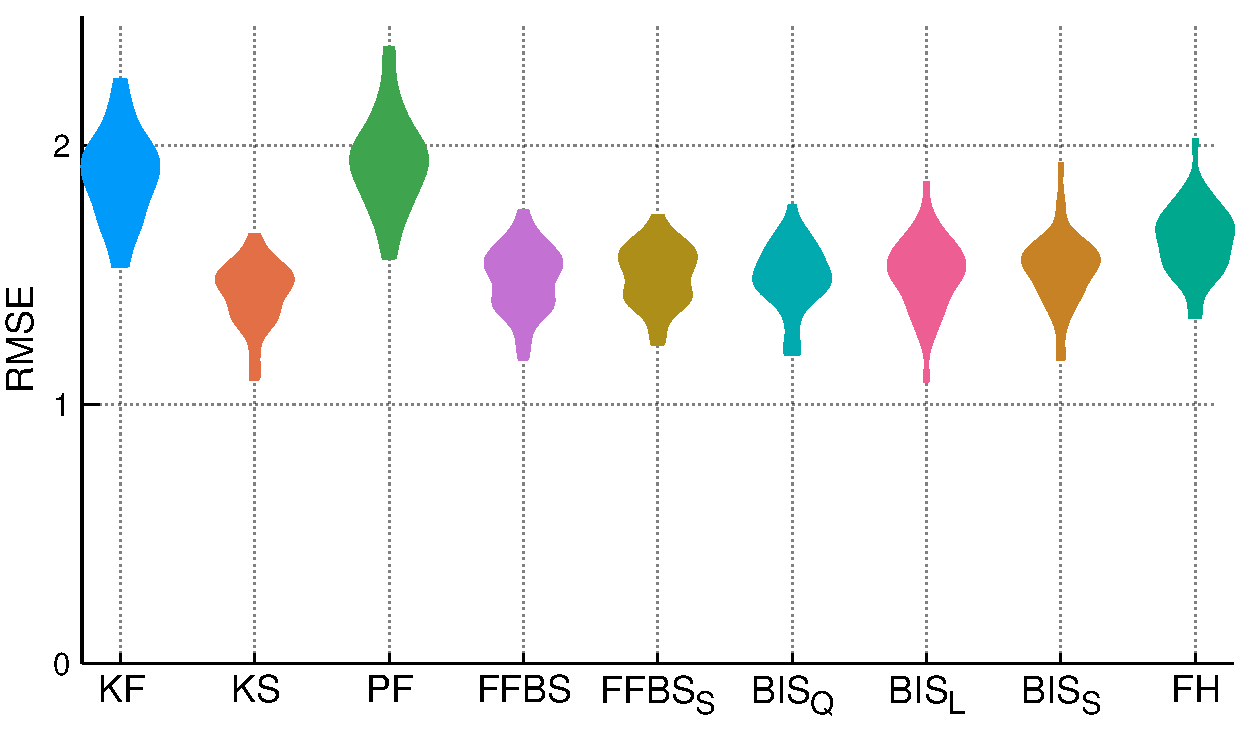
\includegraphics[width=.75\textwidth]{figures/tfs/comparison_caseA}
\caption{\label{comp-smoothing-A}Violin plots comparing the RMSE of the algorithms in \emph{case A} over 50 runs. As expected the optimal Kalman smoother tends to perform best, the FFBS and all BIS have comparable performances while the FH underperforms.}
\end{figure}

\begin{figure}[!h]
\center
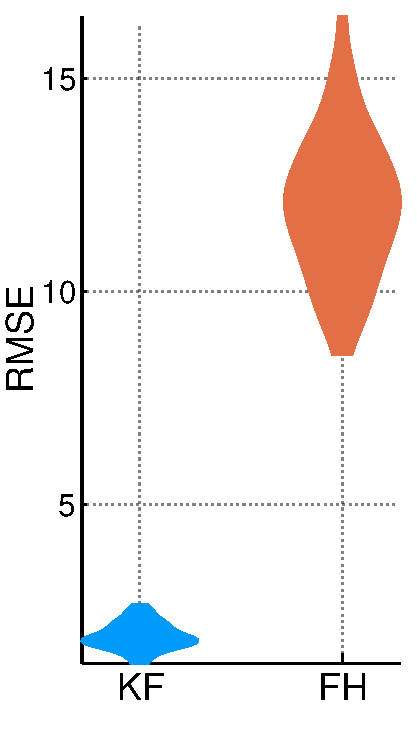
\includegraphics[width=.24\textwidth]{figures/tfs/comparison_caseB_fh+kf}
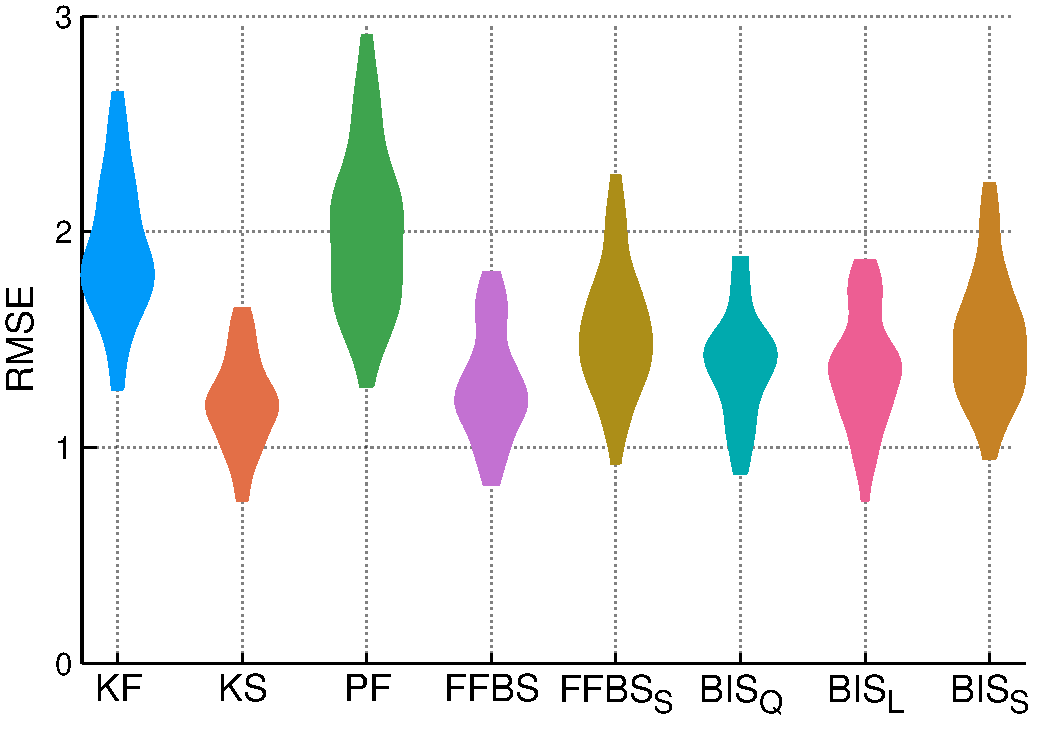
\includegraphics[width=.61\textwidth]{figures/tfs/comparison_caseB}
\caption{\label{comp-smoothing-B}Violin plots comparing the RMSE of the algorithms in \emph{case B} over 50 runs. (left) The FH significantly underperforms  compared to the other algorithms as can be seen compared to the KF which is reproduced on both graph to give an idea of scale (FH is not reproduced on the right as the scale is significantly different from the other algorithms). (right) the other smoothing algorithms offer performances in line with the observations made in case A and do not suffer as much from the decreased noise ratio unlike the FH.}
\end{figure}

%%%%%%%%%%%%%
%\newpage
%%%%%%%%%%%%%

\subsubsection{Model 2 (medium dimensionality)}
In this second example, we consider a model with a 10-dimensional latent space and a 6-dimensional observational space. The matrix $A$ is defined as the identity plus a perturbation matrix $E$ with elements $e_{ij}=\eta_{ij}/5$ with $\eta_{ij}$ drawn from a standard Gaussian. The matrix $B$ has elements $b_{ij}$ drawn from a standard Gaussian. Both matrices $A$ and $B$ are normalised to prevent an explosive behaviour from the HMM. The matrix $Q$ and $R$ have random elements drawn in a similar fashion and both matrices are made positive definite. Both $Q$ and $R$ are normalised and scaled such that $\| Q\| = 1/5$ and $\| R\| = 1/20$. We denote this model LG-10-6 for further reference.

The point of this example is to show that when the particle filter struggles (with a lot of particles with very low weight or, correspondingly, a low ESS) then naturally both version of the FFBS struggle. 
However, the algorithms which apply a resampling of the representation of the particle filter (BIS$_{\text{L}}$ and BIS$_{\text{S}}$) perform very well. Indeed, this resampling allows guiding the smoothing densities to regions of higher expected density (through more concentrated normalising densities $\gamma_{t}$) resulting in better performances overall. The performances are illustrated at figure \ref{comp-model2}.

\begin{figure}[!h]
\center
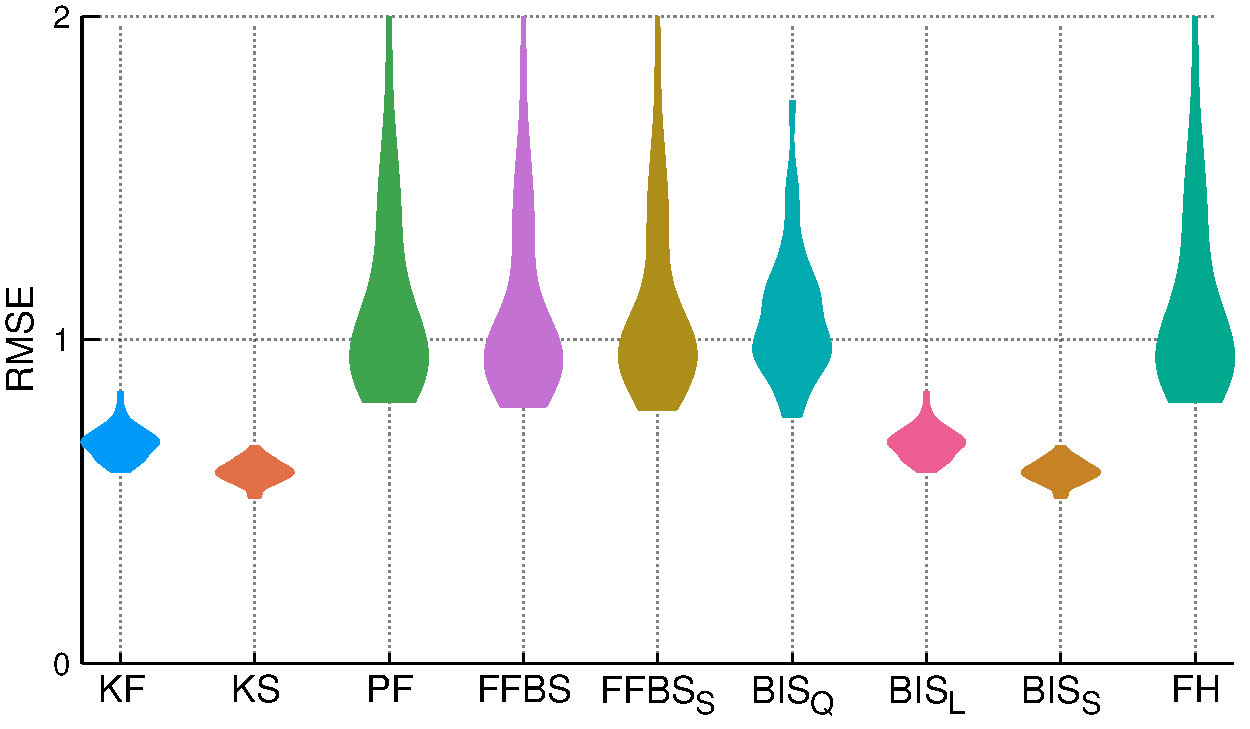
\includegraphics[width=.75\textwidth]{figures/tfs/comparison_mod2}
\caption{\label{comp-model2}Violin plots comparing the RMSE of the algorithms for model LG-10-6 over 50 runs. In this case, the sub-quadratic implementations of the BIS perform outstandingly well compared to the other algorithms which offer little performance gain over simply considering the particle filter.}
\end{figure}

%%%%%%%%
\newpage
%%%%%%%%

\subsection{Nonlinear Gaussian models}
In this point, we show how the sub-quadratic algorithms perform when the dynamic of the HMM is not linear but defined as:
%
\eqa{\syst{ x_{t+1} &=& f_{t}(x_{t}) + \epsilon_{t}\\
		 y_{t+1} &=& g_{t+1}(x_{t+1}) + \eta_{t+1}
}.
}
%
for some sets of functions $\{f_{t}\}_{t=1}^{T}$ and $\{g_{t}\}_{t=1}^{T}$ and with innovation processes $\epsilon_{t}$ and $\eta_{t}$ drawn from centred multivariate Gaussians with covariance matrices $Q$ and $R$.

\subsubsection{Model 3}
This model is drawn from the paper of \citet{arulampalam02} with the dimensionality of both the latent space and the observational space equal to one:
%
\eqa{\syst{
	f_{t}(x) &=& x/2 + 25x(1+x^{2})\inv + 8\cos(1.2t)\\
	g_{t}(x)&=& x^{2}/20\\
},\,\,\text{and}\,\, Q=10,\,\, R=1.
}
%
We call this model NL-1-1 for further reference. We use $N=50$ particles and for $K=100$ time step (as in the original paper) and run the experiments $50$ times with $M=15$ for the sub-quadratic algorithms.

The figure \ref{comp-nl-1} shows the results of the comparison of the RMSE for each algorithm considered. No smoothing algorithm particularly stands out but it shows that the sub-quadratic smoothing algorithms considered do not significantly underperform compared to the full quadratic complexity ones even when the underlying dynamic is non-linear.

\begin{figure}[!h]
\center
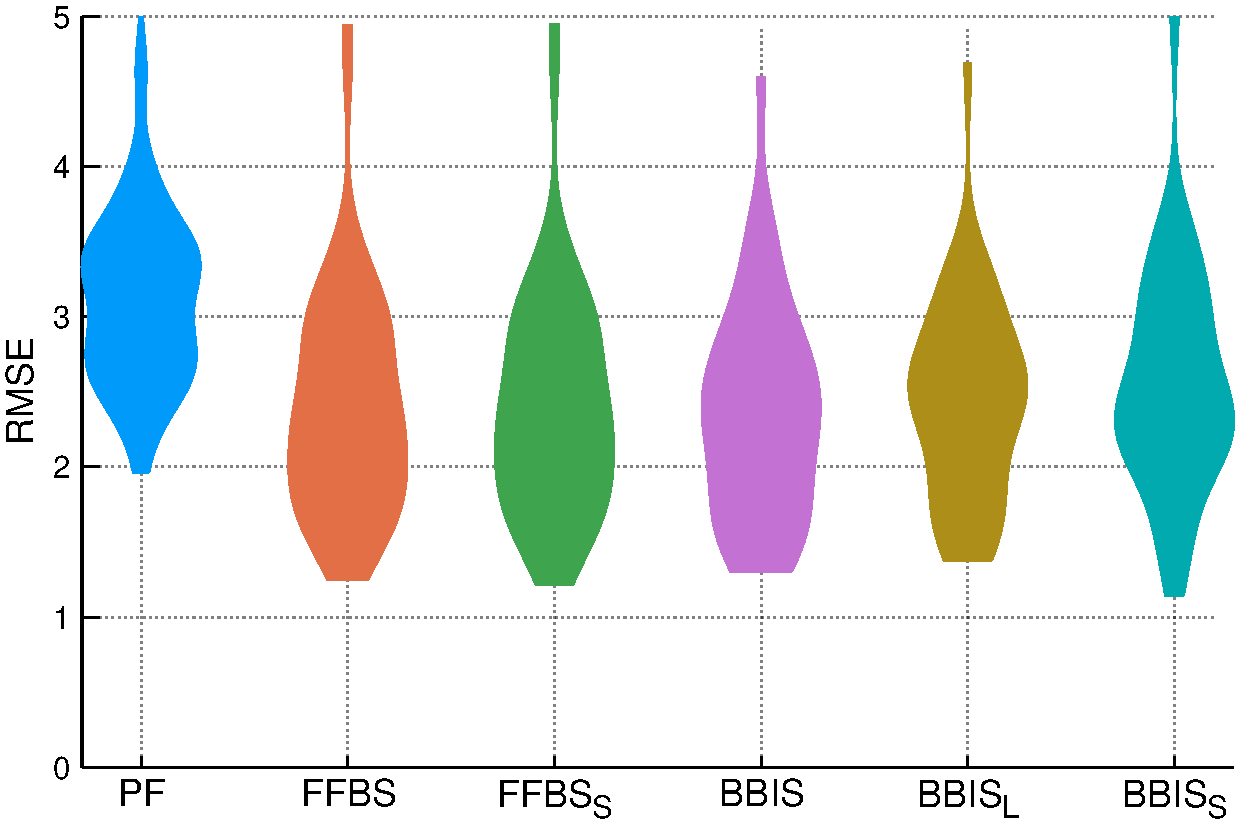
\includegraphics[width=.75\textwidth]{figures/tfs/comp_nl1_N50}
\caption{\label{comp-nl-1}Violin plots comparing the RMSE of the algorithms for model NL-1-1 over 50 runs. In this case, all smoothing algorithms considered offer similar performances showing that sub-quadratic smoothing algorithms can also perform well in the case of a non-linear model.}
\end{figure}

%\subsubsection{Model 4}


\section{Discussion}

In this chapter we suggested and discussed three algorithms with sub-quadratic complexity. 
Two are approximations to the backward information smoother (BIS$_{\text{L}}$, BIS$_{\text{S}}$) using the two filter smoothing algorithm while taking the normalising densities to be approximations of the predictive densities based on a particle filter. 
The last one (FFBS$_{\text{S}}$) is an approximation to the forward filtering backward smoothing algorithm. 

A criticism of the FFBS is that the smoothing step does not sample new particles and just reweighs existing particles which can harm the performance of the resulting estimator. In our experiments however, the FFBS and, more interestingly, its sub-quadratic approximation typically perform well compared to other algorithms. 

The BIS does perform a resampling step in the backward step and uses normalisation densities that are more sensible and typically outperform the default choice suggested in \citep{briers10,fearnhead10}.
However, the optimal backward sampling step is intractable in general and one may have to resort to the bootstrap-BIS as we have in the experiments thereby potentially reducing the advantage of this additional sampling step.

We showed in our experiments that the BIS$_{\text{L}}$ and the BIS$_{\text{S}}$ typically perform on par with the naive implementation. There may be cases in which those algorithms do not perform well but based on the results of the experiments, we would encourage a user to consider the BIS$_{\text{L}}$ as a first smoothing algorithm (provided the dynamic is not linear).

We indicated that the estimators obtained through the BIS$_{\text{L}}$ are not consistent due to the approximation in the sampling of the mixture indices. This, however, seemed to have little impact on the results of the experiments. A possible explanation for this is that, at the regime considered with relatively few particles, all estimators are biased and there is too much variance to significantly distinguish between them. Note however that exploiting these algorithms with significantly more particles (a few orders of magnitude more) requires having to deal with numerical instabilities arising from the representation of the range of weights associated with a large number of particles, and this, even with resampling. This is a known issue, particularly when the dimensionality of the problem is higher and some techniques exist to combat the issue \citep{miguez13}. 

Finally, we have only considered standard multinomial resampling in our algorithms. It may be that alternative resampling procedures such as the ones mentioned in \citet{hol06} lead to improved performances. This could be an avenue for further work.


%Another comment that can be made is that we showed in the previous section that although it was desirable to have $\gamma_{t}\approx \pd_{t}$, it was not necessary as long as $\gamma_{1}=p_{1}$. As shown in \citet{taghavi12}, one could approximate the prediction densities with a mixture of $K$ Gaussians with $K\ll N$ and then consider the full mixture on $KN$ terms instead of a mixture on $N^{2}$ terms. In \citet{taghavi12}, it is shown that mixtures of one or two Gaussians can already provide a good enough approximation to the prediction density in HMM with a simple dynamic. For high-dimensional systems with highly non-Gaussian dynamics however, adjusting a good mixture of a few Gaussians might be expensive and the resulting approximation might be poor.

